\documentclass[11pt]{article}
\usepackage[T1]{fontenc}
\usepackage{lmodern}
\usepackage[top=1.1in,bottom=1.1in,left=1.1in,right=1.1in]{geometry}
\usepackage{amsmath,amssymb,bm}
\usepackage{booktabs}
\usepackage{enumitem}
\usepackage{needspace}
\usepackage{xcolor}
\usepackage{tikz}
\usetikzlibrary{arrows.meta,positioning,calc}
\usepackage{setspace}
\usepackage[colorlinks=true,linkcolor=black,urlcolor=blue]{hyperref}
\setstretch{1.15}
\setlength{\parindent}{0pt}
\setlength{\parskip}{6pt}
\DeclareMathOperator{\Cov}{Cov}
\DeclareMathOperator{\Var}{Var}
\newcommand{\E}{E}
\newcommand{\indep}{\perp\!\!\!\perp}
\definecolor{dukeblue}{RGB}{0,83,155}
\definecolor{accent}{RGB}{200,78,0}
\tikzset{
  dag/.style={>=Stealth,thick,
    every node/.style={circle,draw=dukeblue,fill=white,inner sep=1pt,
                       minimum size=9mm,font=\small}},
  unobs/.style={draw=gray,dashed},
  arr/.style={->,dukeblue,thick},
  uarr/.style={->,gray,thick}}
%% answers: blue, indented, set off from the question
\newenvironment{answer}{\par\smallskip
  \begin{list}{}{\leftmargin=1.2em\rightmargin=0pt}\item[]\color{dukeblue}%
  \textbf{Answer.}\ }{\end{list}\smallskip}
\newcommand{\yn}{\hfill\textsc{yes}\quad\textsc{no}}

\begin{document}

\begin{center}
{\LARGE\bfseries SOCIOL 723: Practice Midterm, With Answers\par}
\vspace{0.6em}
{\large\itshape For practice before the in-class midterm on Thursday, October 15\par}
\end{center}
\vspace{0.5em}

\textbf{Instructions.} This practice exam has the same format, length, and level as the
midterm. The midterm is open book and open note, timed (150 minutes), and asks for no
code. It covers Weeks 1--7 and draws on the frames marked with a blue star in the slides.
Where a question asks for sentences, write them as you would in a paper. Show your
arithmetic: a right number with no work earns partial credit only.

\begin{center}
\renewcommand{\arraystretch}{1.15}
\begin{tabular}{c l l c}
\toprule
Part & Format & Weeks & Points \\
\midrule
1 & Five yes-or-no questions & 1--7 & 10 \\
2 & Ten single-choice questions & 1--7 & 30 \\
3 & Three longer questions & 1--2, 3--4, 5 and 7 & 60 \\
Bonus & One derivation & 5--6 & $+5$ \\
\bottomrule
\end{tabular}
\end{center}

\hrulefill

%% =====================================================================
\section*{Part 1: Yes or No}
Circle \textsc{yes} or \textsc{no}. Two points each.

\begin{enumerate}[leftmargin=*,itemsep=6pt]
\item In your sample, the OLS residuals are uncorrelated with $X$. This is evidence that
      $\E[\epsilon_i \mid X_i] = 0$. \yn
\begin{answer}
\textsc{No}. The normal equations force $\sum_i X_i\hat e_i = 0$ in every sample, for every
dataset. A zero correlation between residuals and $X$ is algebra, not evidence.
\end{answer}

\item Heteroskedasticity makes the OLS coefficients biased. \yn
\begin{answer}
\textsc{No}. Under exogeneity OLS stays unbiased. Only the classical standard-error formula
is wrong; the robust (sandwich) formula fixes it.
\end{answer}

\item The likelihood $\mathcal L(\theta; y)$ is a probability distribution over $\theta$. \yn
\begin{answer}
\textsc{No}. It is the density read backwards: data fixed, $\theta$ varying. It does not
integrate to one over $\theta$.
\end{answer}

\item If treatment is assigned by a coin flip, the difference in mean outcomes between the
      treated and the untreated estimates the ATE. \yn
\begin{answer}
\textsc{Yes}. Randomization gives $(Y_i(0), Y_i(1)) \indep D_i$, so the selection-bias term
$\E[Y_i(0)\mid D_i=1] - \E[Y_i(0)\mid D_i=0]$ is zero and ATE $=$ ATT.
\end{answer}

\item With a binary instrument and no defiers, the first stage
      $\E[D_i\mid Z_i=1] - \E[D_i\mid Z_i=0]$ equals the share of compliers. \yn
\begin{answer}
\textsc{Yes}. The first stage is $\Pr(\text{C}) - \Pr(\text{defiers})$, and monotonicity sets
the second term to zero.
\end{answer}
\end{enumerate}

\newpage
%% =====================================================================
\section*{Part 2: Single Choice}
Circle one letter. Three points each.

\begin{enumerate}[leftmargin=*,itemsep=8pt]
\item A researcher regresses children's test scores on neighborhood poverty and omits
      parental income. Parental income raises test scores, and it is lower in poorer
      neighborhoods. The short regression's poverty coefficient is
      \begin{enumerate}[label=(\Alph*),itemsep=0pt]
      \item biased downward: poverty looks more harmful than it is.
      \item biased upward: poverty looks less harmful than it is.
      \item unbiased, because parental income only affects the outcome.
      \item impossible to sign without the data.
      \end{enumerate}
\begin{answer}
(A). Bias $= \beta_2\,\delta_1$ with $\beta_2 > 0$ (income raises scores) and $\delta_1 < 0$
(income is lower where poverty is higher): the bias is negative.
\end{answer}

\item Students sit in 40 schools, and the treatment was assigned by school. A pairs
      bootstrap that resamples \emph{students} gives a standard error of 0.8. The right
      bootstrap
      \begin{enumerate}[label=(\Alph*),itemsep=0pt]
      \item resamples whole schools with replacement, each bringing all its students.
      \item resamples students, but with $B = 5{,}000$ instead of $1{,}000$.
      \item resamples students within each school.
      \item is not needed: the pairs bootstrap is already heteroskedasticity-robust.
      \end{enumerate}
\begin{answer}
(A). Resample the units the assignment lottery ran over. Resampling students copies the
too-small standard error of the naive formula.
\end{answer}

\item Five independent Poisson counts: $2, 5, 1, 4, 3$. The MLE $\hat\theta$ and its
      standard error are
      \begin{enumerate}[label=(\Alph*),itemsep=0pt]
      \item $3$ and $0.77$
      \item $3$ and $0.60$
      \item $3$ and $1.73$
      \item $2.5$ and $0.71$
      \end{enumerate}
\begin{answer}
(A). $\hat\theta = \bar y = 15/5 = 3$. Observed information
$-\ell''(\hat\theta) = \sum_i y_i/\hat\theta^2 = 15/9 = 1.67$, so
$\text{SE} = 1/\sqrt{1.67} = 0.77$; equivalently $\sqrt{\hat\theta/n} = \sqrt{3/5}$.
\end{answer}

\item A logit is fitted with and without a block of three dummies, on the same 2,000 rows.
      The log-likelihoods are $-1{,}199.1$ (with) and $-1{,}204.6$ (without). The
      $\chi^2_3$ 5\% cut-off is $7.81$ and $\log 2000 = 7.6$. Which is right?
      \begin{enumerate}[label=(\Alph*),itemsep=0pt]
      \item $LR = 11.0$: reject at 5\%; BIC prefers the model without the block.
      \item $LR = 5.5$: do not reject at 5\%.
      \item $LR = 11.0$: reject at 5\%; BIC prefers the model with the block.
      \item $LR = -11.0$: the smaller model fits better.
      \end{enumerate}
\begin{answer}
(A). $LR = 2[-1199.1 - (-1204.6)] = 11.0 > 7.81$. BIC charges $q\log n = 3 \times 7.6 =
22.8$ for the block, more than the $11.0$ it buys: $BIC_{\text{small}} - BIC_{\text{big}} =
11.0 - 22.8 < 0$.
\end{answer}

\item In a logit of voting ($0/1$), the coefficient on holding a college degree is $0.693$,
      so $e^{0.693} = 2$. Which sentence is correct?
      \begin{enumerate}[label=(\Alph*),itemsep=0pt]
      \item Graduates are twice as likely to vote as non-graduates.
      \item A degree raises the probability of voting by $0.693$.
      \item A degree doubles the odds of voting, other covariates held fixed.
      \item A degree raises the probability of voting by 50 percentage points.
      \end{enumerate}
\begin{answer}
(C). $e^{\beta}$ multiplies the odds. It is not a ratio of probabilities, and the change in
probability depends on where a person starts on the S-curve.
\end{answer}

\item A Poisson regression of the number of arrests shows strong overdispersion. What
      follows?
      \begin{enumerate}[label=(\Alph*),itemsep=0pt]
      \item The coefficients are badly biased and must be discarded.
      \item The coefficients are about right, but the Poisson standard errors are too
            small.
      \item The standard errors are too large, so the tests are conservative.
      \item Nothing: overdispersion only matters for prediction.
      \end{enumerate}
\begin{answer}
(B). The mean is still right, so $\hat{\bm\beta}$ is fine; the Poisson's variance $=$ mean
claim is wrong, so its SEs are too small. Use robust SEs or a negative binomial.
\end{answer}

\item A random-intercept model of math scores for students in schools reports
      $\hat\tau^2 = 4$ (between schools) and $\hat\sigma^2 = 36$ (within schools). The
      intraclass correlation is
      \begin{enumerate}[label=(\Alph*),itemsep=0pt]
      \item $0.10$
      \item $0.11$
      \item $0.33$
      \item $0.90$
      \end{enumerate}
\begin{answer}
(A). $\text{ICC} = \tau^2/(\tau^2+\sigma^2) = 4/40 = 0.10$: 10\% of the unexplained variation
is between schools.
\end{answer}

\needspace{12\baselineskip}
\item Four units:
\begin{center}\small
\renewcommand{\arraystretch}{1.05}
\begin{tabular}{ccccc}
\toprule
Unit & $D_i$ & $Y_i(0)$ & $Y_i(1)$ \\
\midrule
1 & 1 & 3 & 9 \\
2 & 1 & 5 & 9 \\
3 & 0 & 4 & 6 \\
4 & 0 & 2 & 2 \\
\bottomrule
\end{tabular}
\end{center}
      \begin{enumerate}[label=(\Alph*),itemsep=0pt]
      \item ATE $= 3$, ATT $= 5$, naive comparison $= 6$
      \item ATE $= 5$, ATT $= 3$, naive comparison $= 6$
      \item ATE $= 3$, ATT $= 5$, naive comparison $= 5$
      \item ATE $= 4$, ATT $= 5$, naive comparison $= 6$
      \end{enumerate}
\begin{answer}
(A). $\tau_i = 6, 4, 2, 0$. ATE $= 12/4 = 3$; ATT $= (6+4)/2 = 5$. Observed $Y_i = 9, 9, 4,
2$, so naive $= 9 - 3 = 6$ $=$ ATT $+$ selection bias $= 5 + (4 - 3)$.
\end{answer}

\needspace{14\baselineskip}
\item In the DAG below, $D$ is job training, $Y$ is earnings two years later, $X$ is
      earnings before training, $M$ is hours worked after training, and $S$ is whether the
      person is still in the survey at follow-up. To estimate the \emph{total} effect of $D$
      on $Y$, condition on
\begin{center}
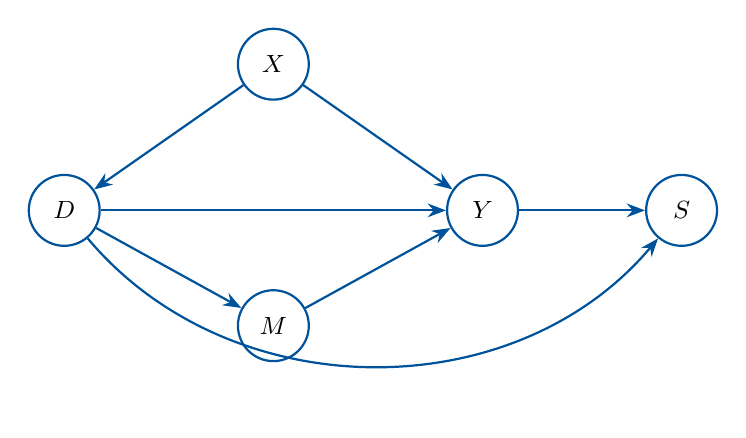
\begin{tikzpicture}[dag,node distance=1.2cm and 2.0cm]
  \node (X) {$X$};
  \node (D) [below left=of X] {$D$};
  \node (Y) [below right=of X] {$Y$};
  \node (M) [below=1.0cm of $(D)!0.5!(Y)$] {$M$};
  \node (S) [right=1.6cm of Y] {$S$};
  \draw[arr] (X) -- (D);
  \draw[arr] (X) -- (Y);
  \draw[arr] (D) -- (Y);
  \draw[arr] (D) -- (M);
  \draw[arr] (M) -- (Y);
  \draw[arr] (Y) -- (S);
  \draw[arr] (D) to[bend right=50] (S);
\end{tikzpicture}
\end{center}
      \begin{enumerate}[label=(\Alph*),itemsep=0pt]
      \item $X$ only.
      \item $X$ and $M$.
      \item $X$ and $S$ (that is, analyze only people still in the survey).
      \item $X$, $M$, and $S$.
      \end{enumerate}
\begin{answer}
(A). $X$ is a confounder (the back door $D \leftarrow X \to Y$). $M$ is a mediator:
conditioning removes part of the effect. $S$ is a collider ($D \to S \leftarrow Y$):
conditioning, including by keeping only respondents still in the survey, opens a
spurious path.
\end{answer}

\item In a cell where the propensity score is $e(x) = 0.8$, weighting for the ATT gives each
      \emph{untreated} unit the weight
      \begin{enumerate}[label=(\Alph*),itemsep=0pt]
      \item $4$
      \item $1.25$
      \item $5$
      \item $0.25$
      \end{enumerate}
\begin{answer}
(A). ATT weights: treated $1$, untreated $e(x)/(1-e(x)) = 0.8/0.2 = 4$, the odds of
treatment. The untreated are reweighted to look like the treated, of whom there are four
per untreated unit in this cell.
\end{answer}
\end{enumerate}

\newpage
%% =====================================================================
\section*{Part 3: Longer Questions}
Twenty points each. Every number below comes from the course's GSS extract or from Lab 7's
data.

%% ---------------------------------------------------------------------
\subsection*{Question 1: Schooling, Parental Education, and Earnings}
The GSS extract has $3{,}509$ full-time workers aged 25--64 (GSS 2010--22). The outcome is
log annual earnings. Three OLS regressions:
\begin{center}\small
\renewcommand{\arraystretch}{1.15}
\begin{tabular}{lccc}
\toprule
 & (1) log earnings & (2) log earnings & (3) parents' education \\
\midrule
years of schooling & $0.1187$ & $0.1099$ & $0.5703$ \\
parents' education (years) & & $0.0154$ & \\
intercept & $8.2307$ & $8.1546$ & $4.9405$ \\
$R^2$ & $0.129$ & $0.132$ & \\
\bottomrule
\end{tabular}
\end{center}
Standard errors for the schooling coefficient in model (2), three ways:
classical $0.0058$; HC3 $0.0064$; clustered on the GSS primary sampling unit ($839$ clusters,
median size four) $0.0065$.

\begin{enumerate}[label=(\alph*),leftmargin=*,itemsep=6pt]
\item Interpret the schooling coefficient in model (1) in one sentence a reader of a
      sociology journal would understand.
\begin{answer}
Among these workers, each additional year of schooling is associated with about $0.119$ log
points, roughly $12\%$, higher annual earnings. It is a description (the best linear
approximation to the CEF), not yet a causal claim.
\end{answer}

\item Use the omitted-variable-bias formula to recover the coefficient in model (1) from
      models (2) and (3). Show the arithmetic, and explain in words why adding parents'
      education lowers the schooling coefficient.
\begin{answer}
Short $=$ long $+$ (effect of omitted) $\times$ (regression of omitted on included):
$0.1099 + 0.0154 \times 0.5703 = 0.1099 + 0.0088 = 0.1187$. Parents' education raises
earnings ($0.0154 > 0$) and moves with own schooling ($0.5703 > 0$), so model (1) credits
schooling with part of the family-background advantage; the bias is positive.
\end{answer}

\item Is $0.1099$ the causal effect of a year of schooling? Name one variable still omitted,
      sign the bias it creates, and say whether a higher $R^2$ would settle the matter.
\begin{answer}
Not without an argument that nothing else confounds schooling and earnings. Ability is the
standard omitted variable: it raises earnings and rises with schooling, so the coefficient
is still overstated. $R^2$ does not help: it answers how well the line fits (Week 1's Q1),
not whether the compared people are comparable (Q2).
\end{answer}

\item Using the HC3 standard error, compute the $t$-statistic and a 95\% confidence
      interval for the schooling coefficient in model (2). Explain why the HC3 and classical
      standard errors differ while the coefficient is the same.
\begin{answer}
$t = 0.1099/0.0064 = 17.2$; interval $0.1099 \pm 1.96 \times 0.0064 = [0.097,\ 0.122]$.
The coefficient comes from the same normal equations either way. The classical formula
pools one $s^2$; HC3 lets each observation carry its own squared residual (inflated by its
leverage), so it is right when the spread of earnings differs across schooling levels.
Heteroskedasticity changes the uncertainty, not the estimate.
\end{answer}

\item The GSS samples areas first and then people within them. Which of the three
      standard errors would you report, and why are the HC3 and clustered numbers so
      close here?
\begin{answer}
The clustered one: cluster at the level of the sampling lottery, the primary sampling unit.
Here the clusters are tiny (median four people), so little within-cluster correlation can
accumulate and the clustered SE barely moves ($0.0065$ vs $0.0064$). Say so rather than
choosing the smaller number.
\end{answer}

\item A colleague suggests adding occupational prestige to model (2) ``to be safe.'' Do you
      agree? Answer with a reason that refers to what the coefficient would then estimate.
\begin{answer}
No. Occupation is a consequence of schooling on the path to earnings, a mediator. Holding it
fixed removes the part of the schooling effect that works through better jobs, so the
coefficient would no longer be the total effect. More controls are not more conservative.
\end{answer}
\end{enumerate}

\newpage
%% ---------------------------------------------------------------------
\subsection*{Question 2: A Logit of Ever Having Married}
Same $3{,}509$ workers; $73\%$ have ever married. A logit of ever married ($0/1$):
\begin{center}\small
\renewcommand{\arraystretch}{1.1}
\begin{tabular}{lrrrr}
\toprule
 & $\hat\beta$ & SE & $z$ & $e^{\hat\beta}$ \\
\midrule
intercept & $-2.2286$ & $0.2791$ & $-7.98$ & \\
years of schooling & $-0.0147$ & $0.0149$ & $-0.99$ & $0.985$ \\
female & $0.0406$ & $0.0836$ & $0.49$ & $1.041$ \\
Black & $-0.9636$ & $0.1066$ & $-9.04$ & $0.382$ \\
age (years) & $0.0864$ & $0.0043$ & $19.91$ & $1.090$ \\
\midrule
log-likelihood & \multicolumn{4}{l}{$-1{,}769.5$} \\
\bottomrule
\end{tabular}
\end{center}
Average marginal effects: age $0.0144$ per year; Black $-0.178$.

\begin{enumerate}[label=(\alph*),leftmargin=*,itemsep=6pt]
\item Write the model twice: once in log-odds form and once in probability form.
\begin{answer}
$\log\dfrac{p_i}{1-p_i} = \beta_0 + \beta_1\,\text{school}_i + \beta_2\,\text{female}_i +
\beta_3\,\text{Black}_i + \beta_4\,\text{age}_i = X_i'\bm\beta$, and
$p_i = \dfrac{e^{X_i'\bm\beta}}{1+e^{X_i'\bm\beta}}$.
\end{answer}

\item Read the Black coefficient on all three scales: log-odds, odds, and probability. Say
      what is wrong with the sentence ``Black workers are $62\%$ less likely to have
      married.''
\begin{answer}
Log-odds: $0.96$ lower, other covariates fixed. Odds: multiplied by $e^{-0.964} = 0.38$.
Probability: on average $17.8$ percentage points lower (the AME). The sentence reads the
odds ratio as a ratio of probabilities; $0.38$ multiplies the odds, and the probability
change depends on where a person sits on the S-curve.
\end{answer}

\item Compute, by hand, the predicted probability of having married for a woman with 16
      years of schooling who is not Black, at age 30 and at age 40.
\begin{answer}
Age 30: $X'\hat\beta = -2.2286 - 0.0147(16) + 0.0406 + 0.0864(30) = 0.169$; odds
$e^{0.169} = 1.18$; $\hat p = 1.18/2.18 = 0.54$. Age 40: add $10 \times 0.0864 = 0.864$,
$X'\hat\beta = 1.033$, odds $2.81$, $\hat p = 0.74$.
\end{answer}

\item For this woman, ten years of age raise the probability by about 20 points. Ten times
      the AME of age is only $14$ points. Explain the difference.
\begin{answer}
The slope of the probability is $\hat p_i(1-\hat p_i)\hat\beta$: steepest at $\hat p = 0.5$.
This woman starts at $0.54$, the steep part of the S-curve. The AME averages the slope over
all $3{,}509$ people, and with $73\%$ married most of them sit higher, where the curve is
flatter.
\end{answer}

\item Adding eight census-region dummies raises the log-likelihood to $-1{,}756.6$. Carry
      out the likelihood-ratio test (the $\chi^2_8$ 5\% cut-off is $15.5$). Then compute
      $BIC_{\text{without}} - BIC_{\text{with}}$ using $\log n = 8.16$, and explain why the
      test and BIC disagree. If region were a confounder of a coefficient you care about,
      would you drop it?
\begin{answer}
$LR = 2[-1756.6 - (-1769.5)] = 25.9 > 15.5$, $p = 0.001$: region matters. BIC:
$LR - q\log n = 25.9 - 8 \times 8.16 = -39.4$, so BIC prefers the model without region.
Eight parameters bought $25.9$ units of fit, about $3.2$ each: too much for chance, too little
for BIC's price of $8.16$ per parameter. A confounder stays regardless: selection criteria
choose descriptions, not identification.
\end{answer}
\end{enumerate}

\newpage
%% ---------------------------------------------------------------------
\subsection*{Question 3: College Proximity as an Instrument (Card 1995)}
Lab 7's data: $3{,}010$ men from the NLS Young Men, first interviewed in 1966. $D$ = years of
schooling; $Y$ = log hourly wage in 1976; $Z = 1$ if the man grew up in a county with a
four-year college ($68\%$ did). All four regressions control for experience, experience
squared, Black, metropolitan residence, and South. HC1 standard errors in parentheses:
\begin{center}\small
\renewcommand{\arraystretch}{1.15}
\begin{tabular}{lcccc}
\toprule
 & OLS of $Y$ on $D$ & first stage, $D$ on $Z$ & reduced form, $Y$ on $Z$ & IV \\
\midrule
estimate & $0.074$ & $0.337$ & $0.045$ & $0.132$ \\
(se) & $(0.004)$ & $(0.081)$ & $(0.016)$ & $(0.049)$ \\
\bottomrule
\end{tabular}
\end{center}
Robust first-stage $F = 17.5$. (Unrounded: reduced form $0.0446$, first stage $0.3373$.)

\begin{enumerate}[label=(\alph*),leftmargin=*,itemsep=6pt]
\item Draw a DAG with $Z$, $D$, $Y$, unmeasured ability $U$, and local labor-market
      conditions $L$. Mark the arrows that must be \emph{absent} for $Z$ to be a valid
      instrument.
\begin{answer}
Arrows present: $Z \to D \to Y$, $U \to D$, $U \to Y$; $L \to Y$ (and possibly $L \to D$).
Must be absent: $Z \to Y$ directly (exclusion), and any common cause of $Z$ and $Y$, such as
$L \to Z$ with $L \to Y$, or $U \to Z$ (independence). The controls (metropolitan, South)
are there to block the $Z \leftarrow L \to Y$ path.
\end{answer}

\item Show that the IV estimate is the ratio of two numbers in the table, and interpret it
      in one sentence.
\begin{answer}
$\hat\beta_{IV} = \text{reduced form}/\text{first stage} = 0.0446/0.3373 = 0.132$. Growing up
near a college raises wages by $4.5\%$ and schooling by a third of a year; scaled up, a year
of schooling raises wages by about $13\%$ for the men whose schooling proximity changed.
\end{answer}

\item State the three IV conditions for this instrument. For each, say whether it can be
      tested, and give one threat specific to college proximity.
\begin{answer}
\textbf{Relevance}: proximity moves schooling. Testable; passes ($0.337$, $F = 17.5$).
\textbf{Independence}: proximity is as good as random given the controls. Not testable;
threat: families who live near colleges differ (richer, more educated parents).
\textbf{Exclusion}: proximity affects wages only through schooling. Not testable; threat:
counties with colleges have better local labor markets that raise wages directly.
\end{answer}

\item Ability bias predicts that OLS overstates the return to schooling, yet IV ($0.132$) is
      almost twice OLS ($0.074$). Give two explanations consistent with valid instruments.
\begin{answer}
(i) \textbf{Measurement error} in reported schooling pulls OLS toward zero; IV is not
affected by classical error in $D$. (ii) \textbf{LATE}: IV estimates the return for compliers,
men whose schooling was moved by having a college nearby, typically from poorer families
facing cost barriers; their return can be higher than the average return OLS summarizes.
(A violated exclusion or weak-instrument bias would also push IV up, but those are failures
of the design, not explanations under valid instruments.)
\end{answer}

\item Treat schooling as ``attended college or not.'' Describe compliers, always-takers, and
      never-takers in this setting, and state monotonicity in words. Is the IV estimate the
      right number for a policy that opens new colleges in counties without one?
\begin{answer}
Compliers attend college only if one is nearby; always-takers attend wherever they grow up;
never-takers do not attend either way. Monotonicity: no one attends \emph{because} there is
no college nearby. For opening new colleges the LATE is close to the right number: the men
such a policy would move are exactly those whose attendance responds to proximity. It is not
the effect for always-takers or for everyone.
\end{answer}

\item The first-stage $F$ of $17.5$ clears the ``$F > 10$'' rule. Should you trust the
      conventional $t$-test of the IV estimate ($t = 2.72$)? What would you report?
\begin{answer}
Not fully. $F > 10$ was derived to keep bias small; for a $t$-test with correct size, Lee et
al.\ (2022) show $F$ must exceed about $104$. At $F = 17.5$ the honest critical value is well
above $1.96$, so report a weak-instrument-robust interval (Anderson--Rubin, or the tF
adjustment), together with the reduced form ($0.045$, $t = 2.72$), which needs no strength
assumption, and the first stage and OLS alongside.
\end{answer}
\end{enumerate}

\newpage
%% =====================================================================
\section*{Bonus: Where the Naive Comparison Goes Wrong}
Five points. Use only the definitions of the ATE, ATT, ATU, and $\pi = \Pr(D_i = 1)$, the
switching equation, and the law of iterated expectations.

\begin{enumerate}[label=(\alph*),leftmargin=*,itemsep=6pt]
\item Prove that $\text{ATE} = \pi\,\text{ATT} + (1-\pi)\,\text{ATU}$.
\item Prove that
\begin{align*}
  \E[Y_i\mid D_i=1] - \E[Y_i\mid D_i=0]
  &= \text{ATE}
  + \underbrace{\E[Y_i(0)\mid D_i=1] - \E[Y_i(0)\mid D_i=0]}_{\text{baseline selection}} \\
  &\quad + \underbrace{(1-\pi)(\text{ATT} - \text{ATU})}_{\text{selection on the effect}} .
\end{align*}
\item Check the identity on the four units of Part 2, Question 8.
\item Show that both selection terms are zero when treatment is randomly assigned.
\end{enumerate}

\begin{answer}
\textbf{(a)} Write $\tau_i = Y_i(1) - Y_i(0)$. By iterated expectations over the two values
of $D_i$,
\begin{align*}
  \text{ATE} = \E[\tau_i]
  &= \Pr(D_i=1)\,\E[\tau_i\mid D_i=1] + \Pr(D_i=0)\,\E[\tau_i\mid D_i=0]
  && \text{\footnotesize iterated exp.} \\
  &= \pi\,\text{ATT} + (1-\pi)\,\text{ATU} .
  && \text{\footnotesize definitions}
\end{align*}
\textbf{(b)} By the switching equation, $Y_i = Y_i(1)$ when $D_i = 1$ and $Y_i = Y_i(0)$ when
$D_i = 0$. Add and subtract $\E[Y_i(0)\mid D_i=1]$:
\begin{align*}
  \E[Y_i\mid D_i=1] - \E[Y_i\mid D_i=0]
  &= \E[Y_i(1)\mid D_i=1] - \E[Y_i(0)\mid D_i=0] \\
  &= \text{ATT} + \E[Y_i(0)\mid D_i=1] - \E[Y_i(0)\mid D_i=0] .
\end{align*}
From (a), $\text{ATT} - \text{ATE} = \text{ATT} - \pi\,\text{ATT} - (1-\pi)\,\text{ATU}
= (1-\pi)(\text{ATT}-\text{ATU})$, so $\text{ATT} = \text{ATE} + (1-\pi)(\text{ATT}-\text{ATU})$.
Substituting this for ATT in the second line gives the identity.
\textbf{(c)} Naive $= 6$; ATE $= 3$; baseline selection $= \tfrac12(3+5) - \tfrac12(4+2) = 1$;
$\pi = 0.5$, ATU $= (2+0)/2 = 1$, so $(1-\pi)(\text{ATT}-\text{ATU}) = 0.5 \times (5-1) = 2$.
$3 + 1 + 2 = 6$. \checkmark
\textbf{(d)} Randomization gives $(Y_i(0),Y_i(1)) \indep D_i$. Then
$\E[Y_i(0)\mid D_i=1] = \E[Y_i(0)\mid D_i=0]$, so baseline selection is zero; and
$\E[\tau_i\mid D_i=1] = \E[\tau_i\mid D_i=0]$, so ATT $=$ ATU and the second term is zero.
\end{answer}

\end{document}
